\documentclass{article}
\usepackage{pgfplots}
\usepackage{tikz}
\usepackage{caption}
\usepackage{graphicx}
\usepackage{times}

\thispagestyle{empty}
\pgfplotsset{compat=1.9}

\begin{document}
\begin{figure}[tb]
\centering
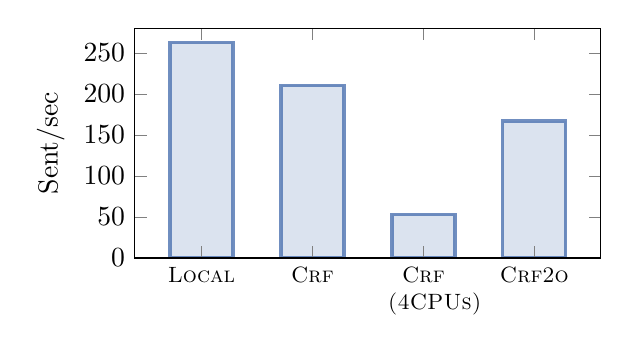
\begin{tikzpicture}
  \begin{axis} [width=7.5cm, height=4.5cm,
    ybar=0pt,
    bar width=0.8cm,
    axis on top,
    enlarge x limits=0.2,
    tick align=inside,
    ymin=0, ymax=280,
    ylabel={Sent/sec},
    ytick={0, 50, ..., 250},
    symbolic x coords={
      \textsc{Local}, \textsc{Crf}, \textsc{Crf (4CPUs)}, \textsc{Crf2o}
    },
    xtick=data,
    x tick label style={rotate=0, text width=0.9cm, font=\footnotesize, align=center},
  ]
  \addplot [draw={rgb,255:red,76; green,114; blue,176},
  very thick,
  draw opacity=0.8,
  fill opacity=0.2, fill={rgb,255:red,76; green,114; blue,176}] coordinates {
    (\textsc{Local}, 262.79)
    (\textsc{Crf}, 210.52)
    (\textsc{Crf (4CPUs)}, 53.291)
    (\textsc{Crf2o}, 166.82)
  };
  \end{axis}
\end{tikzpicture}
\label{fig:ptb-speed}
\end{figure}

\end{document}
